\documentclass{beamer}
\usepackage{amsmath,amssymb,latexsym,array,fancyheadings,mathdots}
\usepackage{algorithm,algorithmic}
\usepackage{hyperref}
\usepackage{color}
\usepackage{tabularx}
\usepackage[all]{xy}
\usepackage{qtree}
\usepackage{gitinfo2}

%% RCS
%\usepackage{rcs}

%% Colors
\definecolor{darkgreen}{rgb}{0,.4,0}
\definecolor{darkred}{rgb}{.5,0,0}
\definecolor{darkmagenta}{rgb}{.5,0,.5}
\definecolor{orange}{rgb}{1,.5,0}
\definecolor{lightblue}{rgb}{0.122,0.016,0.855}
\definecolor{darkocre}{rgb}{0.471,0.298,0.008}

\usetheme{default}

%% New Theorems
\newtheorem{thm}{Theorem}
\newtheorem{exm}[thm]{Example}
\newtheorem{cor}[thm]{Corollary}
\newtheorem{propo}[thm]{Proposition}
\newtheorem{lem}[thm]{Lemma}
\newtheorem{clm}[thm]{Claim}
\newtheorem{exr}[thm]{Exercise}
\newtheorem{dfn}[thm]{Definition}

%% New commands
\newcommand{\classfont}{\mathsf}
\newcommand{\ATM}{\classfont{A}_{\mathrm{TM}}}
\newcommand{\MTF}{\mathrm{MTF}}
\newcommand{\OPT}{\mathrm{OPT}}
\newcommand{\ALG}{\mathrm{ALG}}
\newcommand{\ALGNAIVE}{\mathrm{ALG}_{\text{na{\"\i}ve}}}
\newcommand{\LRU}{\mathrm{LRU}}
\newcommand{\FIFO}{\mathrm{FIFO}}
\newcommand{\FWF}{\mathrm{FWF}}
\newcommand{\LFD}{\mathrm{LFD}}
\newcommand{\true}{\mathsf{T}}
\newcommand{\false}{\mathsf{F}}
\newcommand{\also}{\wedge}
\newcommand{\lra}{\leftrightarrow}
\newcommand{\tc}{\textcolor}
\newcommand{\df}[1]{\textcolor{red}{\em #1}}
\newcommand{\highlight}[1]{\textcolor{orange}{\em #1}}
\newcommand{\hl}[1]{\textcolor{blue}{\em #1}}
\newcommand{\amp}{\texttt{\&}}
\newcommand{\hsh}{\texttt{\#}}
\newcommand{\ra}{\rightarrow}
\newcommand{\longra}{\longrightarrow}
\newcommand{\Ra}{\Rightarrow}
\newcommand{\rab}{{\rightarrow_\beta}}
\newcommand{\srab}{{\rightarrow^*_\beta}}
\newcommand{\aeq}{{=_\alpha}}
\newcommand{\order}{\mathrm{order}}
\newcommand{\rem}{\mathrm{rem}}
\newcommand{\IP}{\mathbf{IP}}
\newcommand{\PSPACE}{\mathbf{PSPACE}}
\newcommand{\thevalue}{\text{value}}
\newcommand{\pol}[1]{\mathbf{#1}}
\newcommand{\enc}{\text{Enc}}
\newcommand{\xor}{\oplus}
\newcommand{\zo}{\{0,1\}}
\newcommand{\SOPT}{S_{\mathrm{opt}}}
\newcommand{\la}{\leftarrow}
\newcommand{\myurl}[1]{\textcolor{darkgreen}{\url{#1}}}
\newcommand{\myhref}[2]{\textcolor{darkgreen}{\href{#1}{#2}}}
\newcommand{\qaccept}{q_{\mathrm{accept}}}
\newcommand{\qreject}{q_{\mathrm{reject}}}
\newcommand{\opt}{\text{\sc Opt}}
\newcommand{\tr}{\mathrm{tr}}
\newcommand{\csanky}{p^{\textsc{csanky}}}
\newcommand{\berk}{p^{\textsc{berk}}}

%% Algorithms package customization
\renewcommand{\algorithmicrequire}{\textbf{Pre-condition:}} 
\renewcommand{\algorithmicensure}{\textbf{Post-condition:}} 
\algsetup{indent=3em}

\input{prooftree}

%% including/excluding pauses
\newcommand{\ifpause}{\iftrue} % for including pauses
%\newcommand{\ifpause}{\iffalse} % for excluding pauses

%% 2nd or 3rd edition
\newif\ifthird
\thirdtrue
%\thirdfalse

%disables usefoottemplate
\setbeamertemplate{navigation symbols}{}
%\setbeamertemplate{footline}% 
%{\strut\quad\tiny 
%\begin{minipage}{3cm}
%Cryptography - Michael Soltys
%\today\ {\tt v\RCSRevision}
%\end{minipage}\hfill
%\insertsection\
%- \insertframenumber/\inserttotalframenumber\quad\strut}

\newcommand{\mytitle}{Welcome}
\newcommand{\mychpnr}{0}
%% Title page contents
\title{Intro to Analysis of Algorithms \\ \mytitle \\  Chapter \mychpnr}
\author{Michael Soltys}
\date{\textcolor{darkgreen}{\tiny\tt 
[ {\bf Git} Date:\gitAuthorDate\ 
Hash:\gitAbbrevHash\ 
Ed:\ifthird
3rd
\else
2nd
\fi]}}
\institute{CSU Channel Islands}

\setbeamertemplate{footline}{
  \colorbox{white}{\color{black}\tt
     \begin{tabularx}{0.97\textwidth}{XXX}
          IAA Chp \mychpnr\ - Michael Soltys \copyright & 
          \hfill\today\ (\gitAbbrevHash; \ifthird ed3\else ed2\fi)
					\hfill\phantom{.} & 
          \hfill\insertsection\ - \insertframenumber/\inserttotalframenumber \\
      \end{tabularx}}}

\begin{document}

\mode<presentation>
{
}

\parskip 8pt

\section{Introduction}

\begin{frame}
\titlepage
\end{frame}


\begin{frame}
{\bf Course}

{\em An Introduction to the Analysis of Algorithms}

\url{https://github.com/michaelsoltys/IAA-Code}

\begin{minipage}{0.4\textwidth}
\raggedright
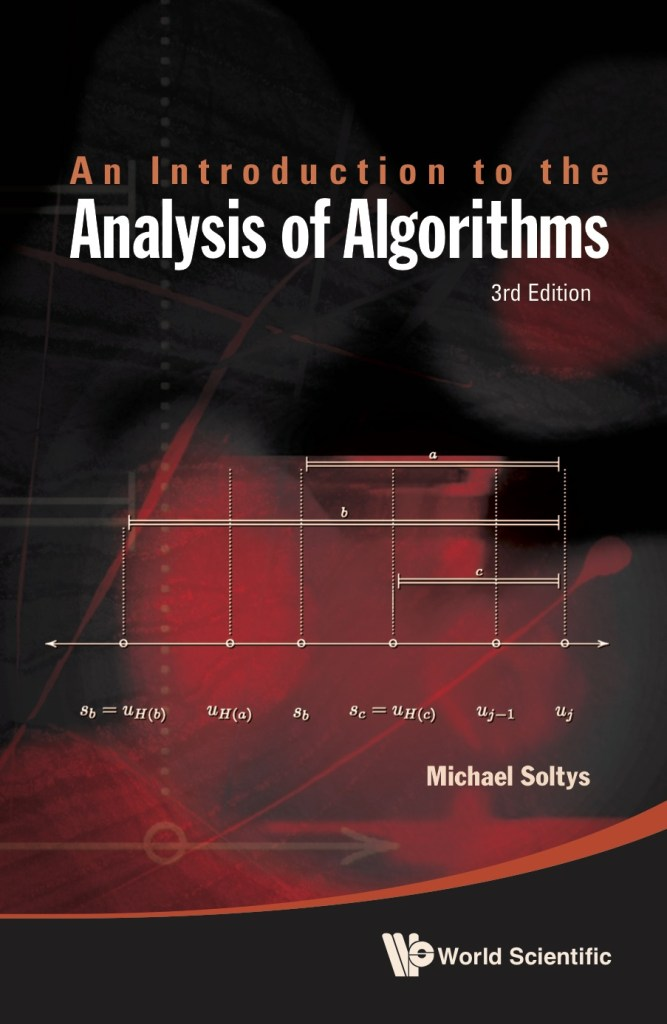
\includegraphics[height=3cm]{Figures/IAA-ed3.jpg}\\
3rd edition
\end{minipage}
\begin{minipage}{0.4\textwidth}
\raggedright
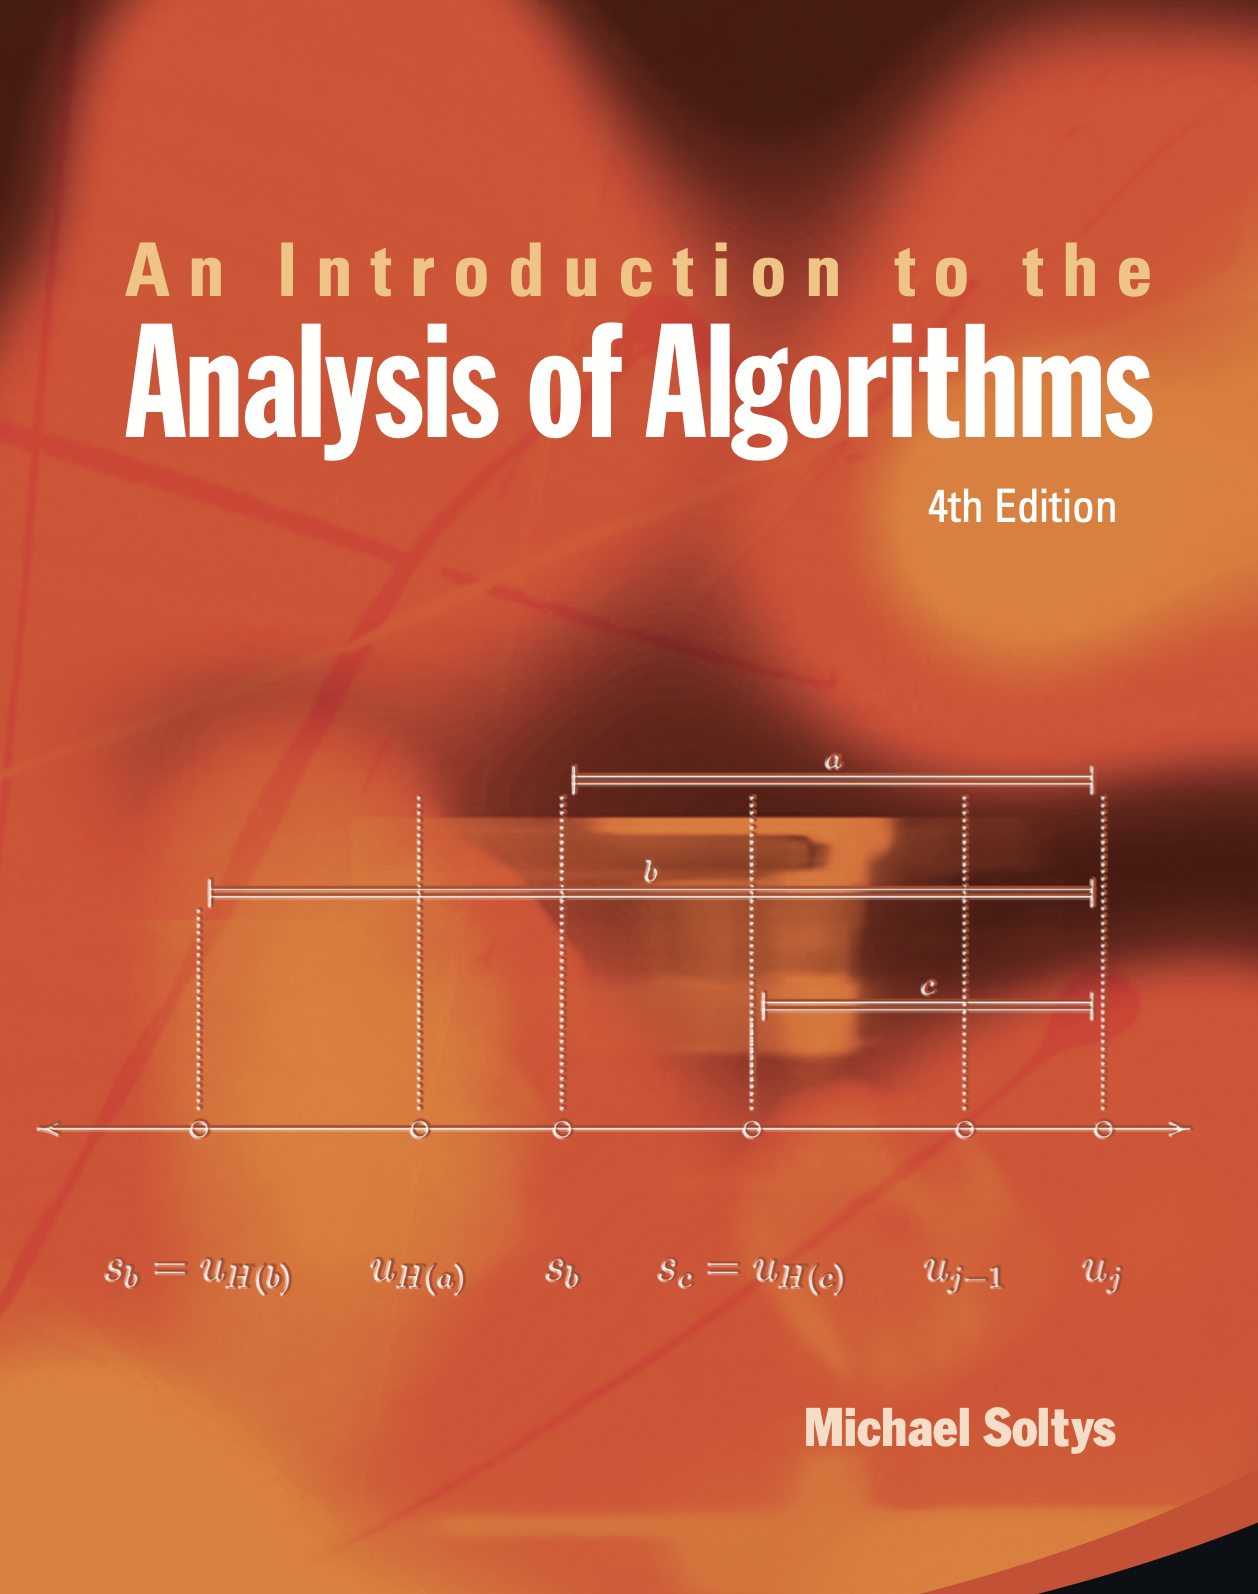
\includegraphics[height=3cm]{Figures/IAA-ed4.png}\\
4th edition
\end{minipage}


\end{frame}

\begin{frame}
{\bf Outline}

\begin{enumerate}
\item  Preliminaries: division, Euclid, Palindromes, etc.; complexity,
and ranking algorithms
\item  Greedy algorithms: spanning trees, jobs, shortest path, Huffman
codes, etc.
\item  Divide and Conquer: mergesort, Savitch's algorithm, etc.
\item  Dynamic Programming: longest monotone subsequence, knapsack
problem, activity selection, etc. \\
\hrulefill
\item  Online Algorithms
\item  Randomized Algorithms
\item  Parallel Algorithms
\item  Machine Learning
\end{enumerate}
\end{frame}

\begin{frame}
{\bf Great introductions to Algorithms}

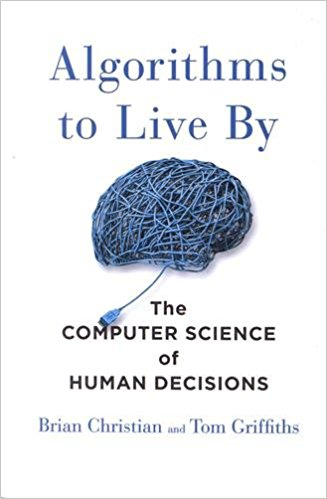
\includegraphics[height=6cm]{Figures/AlgsToLiveBy.jpg}
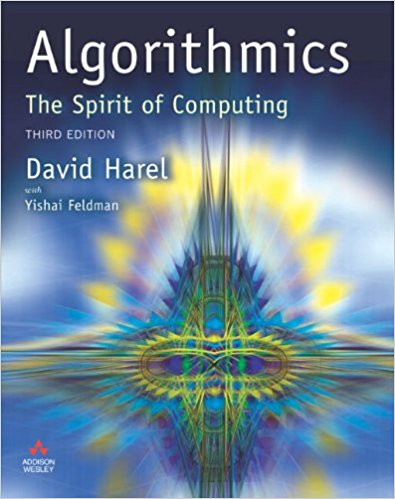
\includegraphics[height=6cm]{Figures/AlgsSpririt.jpg}
\end{frame}

\begin{frame}
{\bf A classic}

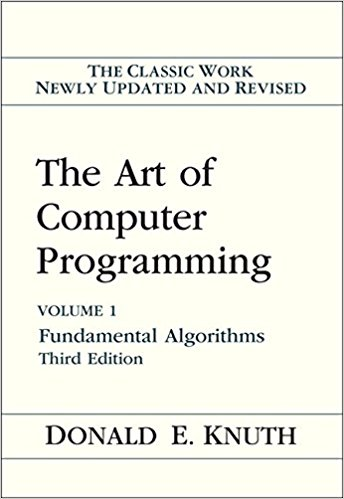
\includegraphics[height=6cm]{Figures/theart.jpg}
\end{frame}

\begin{frame}
{\bf References}

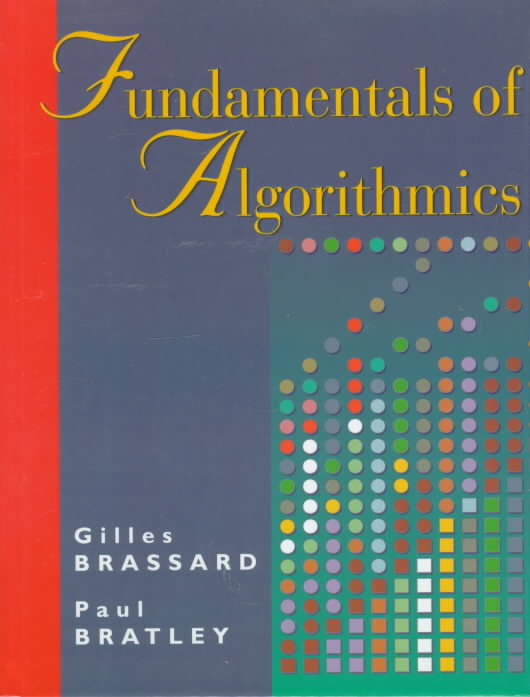
\includegraphics[height=4cm]{Figures/brassard.jpg}
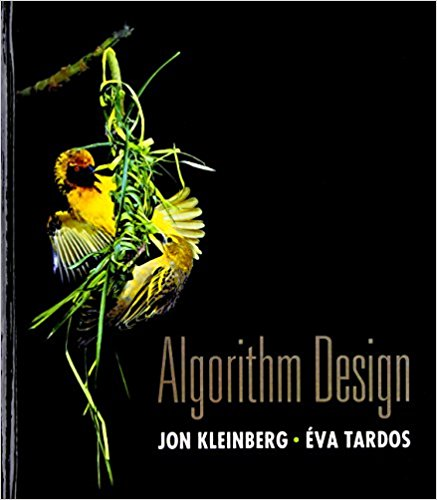
\includegraphics[height=4cm]{Figures/kleinberg.jpg}
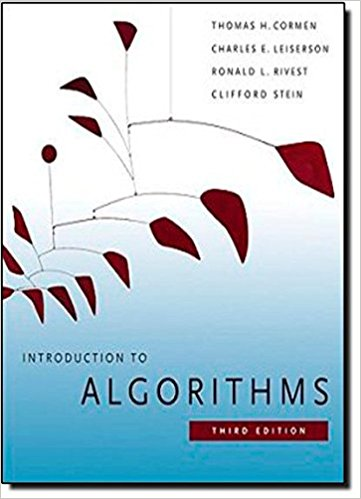
\includegraphics[height=4cm]{Figures/cormen.jpg}

\end{frame}

\begin{frame}
A BBC Documentary by Marcus Du Sautoy

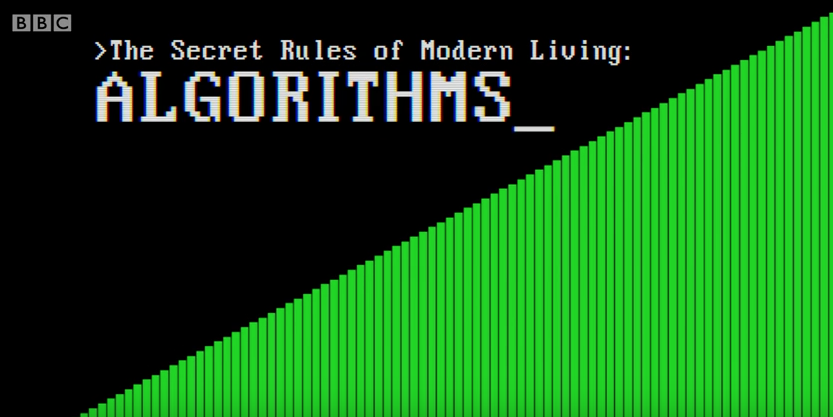
\includegraphics[width=5cm]{Figures/algorithms-bbc.png}

\url{https://youtu.be/kiFfp-HAu64?si=gqN-vBdiZ6u204BF}
\end{frame}

\begin{frame}
{Student Learning Outcome (SLO)}

Measured for the COMP 354 assessment \\
(ABET accreditation requirement)

\bigskip\bigskip

\begin{quote}
\raggedright
Analyze a complex computing problem and to apply principles of
computing and other relevant disciplines to identify solutions.
\end{quote}
\end{frame}

\begin{frame}
{Rubric}
\begin{center}
\tiny
\begin{tabular}{|>{\raggedright\arraybackslash}p{1.8cm}%
|>{\raggedright\arraybackslash}p{1.8cm}%
|>{\raggedright\arraybackslash}p{1.8cm}%
|>{\raggedright\arraybackslash}p{1.8cm}%
|>{\raggedright\arraybackslash}p{1.8cm}|}\hline
{\bf Performance Indicator} &
{\bf Unsatisfactory} & {\bf Developing} & {\bf Satisfactory}
& {\bf Exemplary} \\\hline\hline
1. {\bf Algorithmic design: {\em principle of computing}}
& no understanding of problem, no solution
& problem understood, but solution wrong
& problem understood and a solution given
& problem understood and best solution given \\\hline
2. {\bf Performance analysis: {\em computational complexity}}
& no understanding of what is requested
& understanding of worst-case but no Big-O estimate
& worst-case analysis and a Big-O estimate given
& worst-case analysis resulting in tight Big-O estimate \\\hline
3. {\bf Proof of correctness: {\em Mathematics as other discipline
that helps identify solution}}
& no understanding of how to approach the proof
& providing general direction but no details
& an outline of the proof given and aspects of framework
& a complete proof, with framework of pre/post-condition and
invariants\\\hline
\end{tabular}
\end{center}
\end{frame}

\begin{frame}
\footnotesize
All three rows
will be measured by the corresponding question on the final exam:
\begin{description}
\item[A Design Question:]  A problem is posed, and the students must
choose one of the three basic algorithm design techniques to solve it,
and present the solution in clear and correct pseudo-code.
\item[A Performance Question:]  An algorithm is posed, and the student
must evaluate its time and/or space complexity in terms of worst-case
performance expressed in Big-O notation, and tradeoffs, e.g.,
optimization versus speed, or time resources versus space resources.
\item[Proof of correctness Question:] The student will be given a
problem, and an algorithmic solution will be requested, together with
the proof of correctness of the algorithm; the student will be
required to tie the algorithmic solution to the problem, and to show that
the algorithm solves that problem.
\end{description}
All questions will designate how to measure the answer (as
unsatisfactory, developing, satisfactory or exemplary).
\end{frame}

\end{document}
